\chapter{Simulation}
\label{simulation}

\section{QuISP (Quantum Internet Simulation Package)}

\subsection{Overview}

QuISP \cite{satoh2022quisp} is a quantum network simulator which aims to simulate the behavior of a large-scale quantum network. It is built on top of OMNeT++ \cite{10.5555/1416222.1416290}, which is an event-driven network simulator.
QuISP is built on top of OMNet++ because OMNet++ allows users to define their own networking layers.
QuISP can simulate various types of errors, not only Pauli X error, Pauli Y error and Pauli Z error, but also relaxation error and excitation error.
Physical noise on an actual quantum system with $n$ qubits are usually simulated in the form of a density matrix, which would includes $2^n \times 2^n$ elements and soon becomes intractable as $n$ becomes larger.
QuISP realizes the scalable simulation of quantum network by simulating the physical error using an error probability vector, which would take the following form.

\begin{equation}
  \overrightarrow{\pi}(t) = (\pi_I, \pi_X, \pi_Y, \pi_Z, \pi_R, \pi_E, \pi_L)
\end{equation}
It contains $m+1$ elements (m is the number of simulated error types)
The time evolution of error probability vector is provided by a transition error matrix $Q$.
\begin{equation}
  \overrightarrow{\pi}(t) = \overrightarrow{\pi}(t-1)Q 
\end{equation}

The error probability vector above is the one for a single qubit, so the one for $N$ qubit system contains $N(m+1)$ elements.

\subsection{Hardware Components}

Communication between two quantum nodes is achieved by transmission of photons via an optical fiber, and the fiber is mocked by an object called quantum link.
QuISP supports three main link architecture. 

\subsubsection{Memory-Memory}
The first one is Memory-Memory that two nodes are directly connected via a quantum link and the Bell State Analyzer is equipped in the receiver node.

\subsubsection{Memory-Interference-Memory}
The second one is Memory-Interface-Memory. Both end nodes of a quantum link emits photons to Bell State Analyzer located in the middle. After they become entangled, all the measurements results and required operations are sent back to both nodes.

\subsubsection{Memory-Source-Memory}
The last one Memory-Source-Memory. All the entanglement pairs are both generated and sent from the source of entangled photonic pair states in the middle.

\subsection{Software Components}

\subsubsection{ConnectionManager}

Connection establishment is done when connection manager at the Initiator nodes sends ConnectionSetupRequest to the Responder node and intermediate nodes sends additional information such as those about QNIC.
After that, the connection manager at the responder node sends ConnectionSetupResponse to each node along the path of the connection.

\subsubsection{HardwareMonitor}
HardwareMonitor is the module that collects the information of a quantum link such as fidelity and generation rate and pass those information to the routing daemon and the connection manager.

\subsubsection{BellPairStore}
BellPairStore is the module that stores the entanglement pairs generated from a support node such as a Bell State Analyzer.

\subsubsection{Runtime}
Runtime is the program that executes each RuleSet.

\subsubsection{RuntimeManager}
RuntimeManager is the program that store Runtime for each RuleSet, which is a part of Rule Engine, which is explained in the next section.

\subsubsection{RuleEngine}
RuleEngine is the component that is in charge for executing the given RuleSets and monitor the conditions of physical qubits.


\section{Implementation}

This section discusses the mechanism and required methods that the author implemented in order to realize link management in QuISP.

\subsection{Link Management in QuISP}

\subsubsection{Link Allocation Policy Negotiation}
The first phase of link management in RuleSet-based quantum networking is the negotiation of the next set of RuleSets to execute.
This is triggered by each update in the set of available runtimes, or RuleSets in the Rule Engine, such as the reception of a new RuleSet or the notification of connection teardown, which will be explained in detail in the later section.

First of all, LinkAllocationUpdateMessages are sent to all the neighboring nodes. \ref{algo:sendlau} is the pseudocode of the transmission of those messages.

\begin{algorithm}[H]
  \begin{minipage}{0.8\linewidth}
  \caption{Algorithm For Sending LinkAllocationUpdateMessages}
  \begin{algorithmic}[1]
\Require The address of this node $\text{parent\_address}$
  \Require An array of available runtimes $\text{runtimes}$
  \Require A map of node address of each neighboring nodes and the active link allocation policy $\text{node\_address\_active\_link\_allocations\_map}$
  \Require A map of node address of each neighboring nodes and the next link allocation policy $\text{node\_address\_next\_link\_allocations\_map}$
  \Require A map of node address of each neighboring nodes and a random number $\text{node\_address\_random\_number\_map}$
  \Require A map of node address of each neighboring nodes and whether a LinkAllocationUpdateMessage is sent from this node $\text{node\_address\_lau\_sent\_map}$
  \Function {SendLinkAllocationUpdateMessages}{}
    \State Initialize an array of node addresses of neighboring nodes $\text{partner\_addresses}$
    \ForAll {$\text{runtime} \gets \text{runtimes}$} 
      \ForAll {$\text{partner} \gets$ the list of all the neighboring addresses that $\text{runtime}$ needs to communicate} 
      \State Append $\text{partner}$ to $\text{partner\_addresses}$ if it has not been added
      \EndFor
    \EndFor
    \ForAll {$\text{runtime} \gets \text{runtimes}$} 
      \ForAll {$\text{partner} \gets$ the list of all the neighboring addresses that $\text{runtime}$ needs to communicate} 
      \State Initialize an array for RuleSet IDs in the active link policy $\text{active\_link\_allocations}$
        \If {$\text{partner}$ is a part of the key of $\text{node\_address\_active\_link\_allocations\_map}$}
          \ForAll {$\text{active\_link\_allocation} \gets \text{node\_address\_active\_link\_allocations\_map[partner]}$}
            \State Append $\text{active\_link\_allocation}$ to $\text{active\_link\_allocations}$
          \EndFor
        \EndIf
        \algstore{hoge}
      \end{algorithmic}
    \end{minipage}
    \end{algorithm}

    \begin{algorithm}[H]    
      \begin{minipage}{0.8\linewidth}               
      \begin{algorithmic}[1]
        \algrestore{hoge}
      \State Initialize an array for RuleSet IDs in the next link policy $\text{next\_link\_allocations}$
        \If {$\text{partner}$ is a part of the key of $\text{node\_address\_next\_link\_allocations\_map}$}
          \ForAll {$\text{next\_link\_allocation} \gets \text{node\_address\_next\_link\_allocations\_map[partner]}$}
            \State Append $\text{next\_link\_allocation}$ to $\text{next\_link\_allocations}$
          \EndFor
        \EndIf
        \ForAll {$\text{active\_link\_allocation} \gets \text{active\_link\_allocations}$}
          \State{Append $\text{active\_link\_allocation}$ to $\text{node\_address\_active\_link\_allocations\_map[partner]}$}
        \EndFor
        \ForAll {$\text{next\_link\_allocation} \gets \text{next\_link\_allocations}$}
          \State{Append $\text{next\_link\_allocation}$ to $\text{node\_address\_next\_link\_allocations\_map[partner]}$}
        \EndFor
      \EndFor
      \ForAll {$\text{partner\_address} \gets \text{partner\_addresses}$}
        \State Initialize an new LinkAllocationUpdateMessage $\text{pkt}$
        \State The source address of $\text{pkt} \gets \text{parent\_address}$ 
        \State The target address of $\text{pkt} \gets \text{partner\_address}$ 
        \ForAll {$\text{active\_link\_allocation} \gets \text{node\_address\_active\_link\_allocations\_map[partner]}$}
          \State Append $\text{active\_link\_allocation}$ to activeLinkAllocations of $\text{pkt}$
        \EndFor
        \ForAll {$\text{next\_link\_allocation} \gets \text{node\_address\_next\_link\_allocations\_map[partner]}$}
          \State Append $\text{next\_link\_allocation}$ to nextLinkAllocations of $\text{pkt}$
        \EndFor
        \State {Initialize a random integer $\text{rand\_number}$}
        \State The random number of $\text{pkt} \gets \text{rand\_number}$ 
        \State $\text{node\_address\_random\_number\_map[partner\_address]} \gets \text{rand\_number}$
        \State $\text{node\_address\_lau\_sent\_map[partner\_address]} \gets$ True
        \State Send $\text{pkt}$
      \EndFor
    \EndFor
  \EndFunction
  \end{algorithmic}
  \label{algo:sendlau}
\end{minipage}
\end{algorithm}

If the RuleEngine receives an incoming LinkAllocationUpdateMessage, it has to store the information for the further negotiation.
\begin{algorithm}[H]  
  \begin{minipage}{0.8\linewidth}
  \caption{Algorithm For Storing the Information of an Incoming LinkAllocationUpdateMessage}                 
  \begin{algorithmic}[1]
    \Require An incoming LinkAllocationUpdateMessage $\text{pkt}$
    \Require  A map of node address of each neighboring nodes and the incoming random number $\text{node\_address\_incoming\_random\_number\_map}$
    \Require  A map of node address of each neighboring nodes and the incoming active link allocation policy $\text{node\_address\_incoming\_active\_link\_allocations\_map}$
    \Require  A map of node address of each neighboring nodes and the incoming next link allocation policy $\text{node\_address\_incoming\_next\_link\_allocations\_map}$
    \Require  A map of node address of each neighboring nodes and whether the RuleSet received LinkAllocationUpdateMessage $\text{node\_address\_lau\_received\_map}$
    \State $\text{src\_addr} \gets$ the source address of $\text{pkt}$
    \State $\text{random\_number} \gets$ the random number of $\text{pkt}$
    \State $\text{node\_address\_incoming\_random\_number\_map[src\_addr]} \gets \text{random\_number}$
    \State $\text{incoming\_active\_link\_allocations\_count} \gets$ the number of RuleSets in the active link allocation policy
    \For{$\text{i} \gets 0$ to $\text{incoming\_active\_link\_allocations\_count}$}  
      \State $\text{incoming\_active\_link\_allocation} \gets$ ith element of the ActiveLinkAllocations of $\text{pkt}$
      \State Append $\text{incoming\_active\_link\_allocation}$ to $\text{node\_address\_incoming\_active\_link\_allocations\_map[src\_addr]}$
    \EndFor
    \State $\text{incoming\_next\_link\_allocations\_count} \gets$ the number of RuleSets in the next link allocation policy
    \For{$\text{i} \gets 0$ to $\text{incoming\_next\_link\_allocations\_count}$}  
      \State $\text{incoming\_next\_link\_allocation} \gets$ ith element of the NextLinkAllocations of $\text{pkt}$
      \State Append $\text{incoming\_next\_link\_allocation}$ to $\text{node\_address\_incoming\_next\_link\_allocations\_map[src\_addr]}$
    \EndFor
    \State $\text{node\_address\_lau\_received\_map[src\_addr]} \gets$ True
  \end{algorithmic}
\end{minipage}
\end{algorithm}

If both the incoming and outgoing LinkAllocationUpdateMessages have the same random numbers, the negotiation will be rejected by sending a RejectLinkAllocationUpdateMessage to each other.
\begin{algorithm}[H]  
  \begin{minipage}{0.8\linewidth}
  \caption{Algorithm For Sending a RejectLinkAllocationUpdateMessage}             
  \begin{algorithmic}[1]
    \Require The address of the this node $\text{this\_address}$      
    \Require The address of the destination node $\text{dest\_address}$    
    \State Initialize a new RejectLinkAllocationUpdateMessage $\text{pkt}$
    \State The source address of $\text{pkt} \gets \text{this\_address}$
    \State The destination address of $\text{pkt} \gets \text{dest\_address}$
    \State Send $\text{pkt}$
  \end{algorithmic}
\end{minipage}
\end{algorithm}

After exchanging LinkAllocationUpdateMessages, each pair of nodes need to synchronize the contents and their order of the next link allocation policy.
The policy from the LinkAllocationUpdateMessage with the bigger random value will be prioritized.

\begin{algorithm}[H]  
  \begin{minipage}{0.8\linewidth}
  \caption{Algorithm For Synchronizing the Link Allocation Policy}                 
  \begin{algorithmic}[1]
    \Require The address of the destination node $\text{dest\_address}$
    \Require A map of node address of each neighboring nodes and the incoming random number $\text{node\_address\_incoming\_random\_number\_map}$
    \Require A map of node address of each neighboring nodes and the random number in this node $\text{node\_address\_random\_number\_map}$
    \Require  A map of node address of each neighboring nodes and whether the RuleSet sent BarrierMessage $\text{node\_address\_barrier\_sent\_map}$
    \Require  A map of node address of each neighboring nodes and whether the RuleSet received BarrierMessage $\text{node\_address\_barrier\_received\_map}$
    \State $\text{incoming\_random\_number} \gets \text{node\_address\_incoming\_random\_number\_map[dest\_address]}$
    \State $\text{random\_number} \gets \text{node\_address\_random\_number\_map[dest\_address]}$
    \If{$\text{incoming\_random\_number} == \text{random\_number}$}
      \State $\text{Send a RejectLinkAllocationUpdateMessage}$
    \ElsIf{$\text{incoming\_random\_number} > \text{random\_number}$}
      \State $\text{node\_address\_incoming\_random\_number\_map[dest\_address]} \gets \text{node\_address\_random\_number\_map[dest\_address]}$
      \State $\text{node\_address\_barrier\_sent\_map[dest\_address]} \gets \text{False}$
      \State $\text{node\_address\_barrier\_received\_map[dest\_address]} \gets \text{False}$
    \EndIf
  \end{algorithmic}
\end{minipage}
\end{algorithm}

\subsubsection{Link Allocation Timing Negotiation}

After the next link allocation policy is synchronized between two neighboring nodes, it is time to determine when to update the link allocation policy.
\begin{algorithm}[H]  
  \begin{minipage}{0.8\linewidth}
  \caption{Algorithm For Sending a BarrierMessage}             
  \begin{algorithmic}[1]
    \Require The address of the this node $\text{this\_address}$      
    \Require The address of the destination node $\text{dest\_address}$    
    \State Initialize a new BarrierRequest $\text{pkt}$
    \State The source address of $\text{pkt} \gets \text{this\_address}$
    \State The destination address of $\text{pkt} \gets \text{dest\_address}$
    \State $\text{sequence\_number} \gets$ the smallest value among sequence numbers of the available link Bell pairs
    \State The sequence number of $\text{pkt} \gets \text{sequence\_number}$
    \State Send $\text{pkt}$
  \end{algorithmic}
\end{minipage}
\end{algorithm}

\begin{algorithm}[H]  
  \begin{minipage}{0.8\linewidth}
  \caption{Algorithm For Storing Information About the Incoming BarrierMessage}                 
  \begin{algorithmic}[1]
  \Require The incoming BarrierMessage $\text{pkt}$
    \Require A map of node address of each neighboring nodes and the smallest sequence number in this node $\text{node\_address\_barrier\_sequence\_number\_map}$
    \Require A map of node address of each neighboring nodes and whether the RuleSet received BarrierMessage $\text{node\_address\_barrier\_received\_map}$
    \State $\text{sequence\_number} \gets$ the smallest value among sequence numbers of the available link Bell pairs
    \State $\text{node\_address\_incoming\_sequence\_number\_map[src\_addr]} \gets \text{sequence\_number}$
  \end{algorithmic}
\end{minipage}
\end{algorithm}

\begin{algorithm}[H]  
  \begin{minipage}{0.8\linewidth}
  \caption{Algorithm For Synchronizing the Next Sequence Number}                 
  \begin{algorithmic}[1]
    \Require The node address of one of the neighboring nodes $\text{src\_address}$
    \Require A map of node address of each neighboring nodes and the smallest sequence number in this node $\text{node\_address\_sequence\_number\_map}$
    \Require A map of node address of each neighboring nodes and the incoming smallest sequence number $\text{node\_address\_incoming\_sequence\_number\_map}$
    \State $\text{sequence\_number} \gets \text{node\_address\_sequence\_number\_map[src\_address]}$
    \State $\text{incoming\_sequence\_number} \gets \text{node\_address\_incoming\_sequence\_number\_map[src\_address]}$
    \If {$\text{incoming\_sequence\_number} > \text{sequence\_number}$}
      \State $\text{node\_address\_sequence\_number\_map[src\_addr]} \gets \text{incoming\_sequence\_number}$
    \EndIf
  \end{algorithmic}
\end{minipage}
\end{algorithm}

\subsubsection{Link Management in QuISP}

Allocation of link Bell pairs starts after two neighboring nodes coordinates the first sequence number to start applying the new link allocation policy.
Release of link Bell pairs that were allocated to the terminated connection will be performed after the termination of execution of the associated RuleSet.

\begin{algorithm}[H]  
  \begin{minipage}{0.8\linewidth}
  \caption{Algorithm For Allocating Link Bell pairs}                 
  \begin{algorithmic}[1]
    \Require The QNIC type $\text{qnic\_type}$
    \Require The QNIC index $\text{qnic\_index}$
    \Require The first sequence number $\text{first\_sequence\_number}$
    \State Initialize a map of node addresses of neighboring nodes and the indices of Runtimes $\text{partner\_addr\_runtime\_indices\_map}$
    \State $\text{index} \gets$ 0
    \ForAll {$\text{runtime} \gets \text{runtimes}$}
      \State $\text{partners} \gets$ the addresses of all nodes that $\text{runtime}$ needs to communicate
      \ForAll {$\text{partner} \gets \text{partners}$} 
        \State Append $\text{partner}$ to $\text{partner\_addr\_runtime\_indices\_map[partner]}$
      \EndFor
      \State $\text{index} \gets \text{index + 1}$
    \EndFor

    \ForAll {$\text{[partner\_addr, value]} \gets \text{partner\_addr\_runtime\_indices\_map}$}
      \State $\text{runtime\_indices} \gets \text{partner\_addr\_runtime\_indices\_map[partner\_addr]}$
      \State $\text{bell\_pair\_range} \gets$ the list of Bell pairs on the side of this node
      \State $\text{bell\_pair\_num} \gets$ 0
      \ForAll {$\text{bell\_pair} \gets \text{bell\_pair\_range}$}
        \State $\text{bell\_pair\_num} \gets \text{bell\_pair\_num + 1}$
      \EndFor
      \State  Initialize a map of Runtime indices and the number of Bell pairs $\text{runtime\_index\_bell\_pair\_number\_map}$
      \State $\text{number} \gets$ 0
      \ForAll {$\text{bell\_pair} \gets \text{bell\_pair\_range}$}
        \State $\text{sequence\_number} \gets \text{sequence\_number of bell\_pair}$
        \If {$\text{first\_sequence\_number} <= \text{sequence\_number}$}
          \State $\text{qubit\_record} \gets$ The object of the physical qubit in $\text{bell\_pair}$
          \If {$\text{qubit\_record}$ is not allocated}
            \State $\text{qubit\_record.is\_allocated} \gets$ True
            \State $\text{index} \gets \lfloor \text{number} \times \text{the size of runtime\_indices / bell\_pair\_num} \rfloor$
            \State $\text{i} \gets \text{runtime\_indices[index]}$
            \State Allocate $\text{qubit\_record}$ to the ith Runtime
            \If {$i$ is a part of the key list of $\text{runtime\_index\_bell\_pair\_number\_map}$}
              \State $\text{runtime\_index\_bell\_pair\_number\_map[runtime\_index]} \gets \text{runtime\_index\_bell\_pair\_number\_map[runtime\_index] + 1}$
            \Else
              \State $\text{runtime\_index\_bell\_pair\_number\_map[runtime\_index]} \gets$ 0
            \EndIf
            \algstore{hoge}
          \end{algorithmic}
        \end{minipage}
        \end{algorithm}
    
        \begin{algorithm}[H]    
          \begin{minipage}{0.8\linewidth}               
          \begin{algorithmic}[1]
            \algrestore{hoge}
          \EndIf
        \EndIf
        \State $\text{number} \gets \text{number + 1}$
      \EndFor
    \EndFor
  \end{algorithmic}
\end{minipage}
\end{algorithm}

\begin{algorithm}[H]  
  \begin{minipage}{0.8\linewidth}
  \caption{Algorithm For Releasing Link Bell pairs}                 
  \begin{algorithmic}[1]
    \Require The QNIC type $\text{qnic\_type}$
    \Require The QNIC index $\text{qnic\_index}$
    \Require The first sequence number $\text{first\_sequence\_number}$
    \Require A map of sequence numbers of Bell pairs and associated RuleSet IDs $\text{sequence\_number\_ruleset\_id\_map}$
    \State Initialize a map of node addresses of neighboring nodes and the indices of terminated Runtimes $\text{partner\_addr\_terminated\_runtime\_indices\_map}$
    \State $\text{index} \gets$ 0
    \State $\text{terminated\_runtimes} \gets$ the array of terminated runtime from RuntimeManager
    \ForAll {$\text{terminated\_runtime} \gets \text{terminated\_runtimes}$}
      \State $\text{partners} \gets$ the addresses of all nodes that $\text{terminated\_runtime}$ needs to communicate
      \ForAll {$\text{partner} \gets \text{partners}$} 
        \State Append $\text{partner}$ to $\text{partner\_addr\_terminated\_runtime\_indices\_map[partner]}$
      \EndFor
      \State $\text{index} \gets \text{index + 1}$
    \EndFor

    \ForAll {$\text{[partner\_addr, value]} \gets \text{partner\_addr\_terminated\_runtime\_indices\_map}$}
      \State $\text{runtime\_indices} \gets \text{partner\_addr\_terminated\_runtime\_indices\_map[partner\_addr]}$
      \State $\text{bell\_pair\_range} \gets$ the list of Bell pairs on the side of this node
      \ForAll {$\text{bell\_pair} \gets \text{bell\_pair\_range}$}
        \State $\text{sequence\_number} \gets \text{sequence\_number of bell\_pair}$
          \State $\text{qubit\_record} \gets$ The object of the physical qubit in $\text{bell\_pair}$
          \State $\text{ruleset\_id} \gets \text{sequence\_number\_ruleset\_id\_map[sequence\_number]}$
          \If {$\text{qubit\_record}$ is already allocated}
            \State $\text{qubit\_record.is\_allocated} \gets$ False
            \State Reinitialize the qubit record
            \If {$\text{qubit\_record}$ is already allocated}
              \If {$\text{qubit\_record}$ is busy}
                \State $\text{qubit\_record.is\_busy} \gets$ False
              \EndIf
              \algstore{hoge}
            \end{algorithmic}
          \end{minipage}
          \end{algorithm}

          \begin{algorithm}[H]    
            \begin{minipage}{0.8\linewidth}               
            \begin{algorithmic}[1]
              \algrestore{hoge}
              \ForAll {$\text{terminated\_runtime} \gets \text{terminated\_runtimes}$}
                \If {ID of $\text{terminated\_runtime}$ is $\text{ruleset\_id}$}
                  \State Release $\text{qubit\_record}$ 
                  \State $\text{runtime\_index} \gets \text{sequence\_number\_runtime\_index\_map[sequence\_number]}$
                  \State $\text{runtime\_index\_bell\_pair\_number\_map[runtime\_index]} \gets \text{runtime\_index\_bell\_pair\_number\_map[runtime\_index] - 1}$;
                \EndIf
              \EndFor
            \EndIf
          \EndIf
      \EndFor
    \EndFor
  \end{algorithmic}
\end{minipage}
\end{algorithm}


\subsection{Relationship with Connection Management}
\subsubsection{Connection Setup}

There are three steps for connection setup in RuleSet-based quantum networking. 
The first one is the transmission of a ConnectionSetupRequest from the Initiator to the Responder.
\begin{figure}[H]
  \centerline{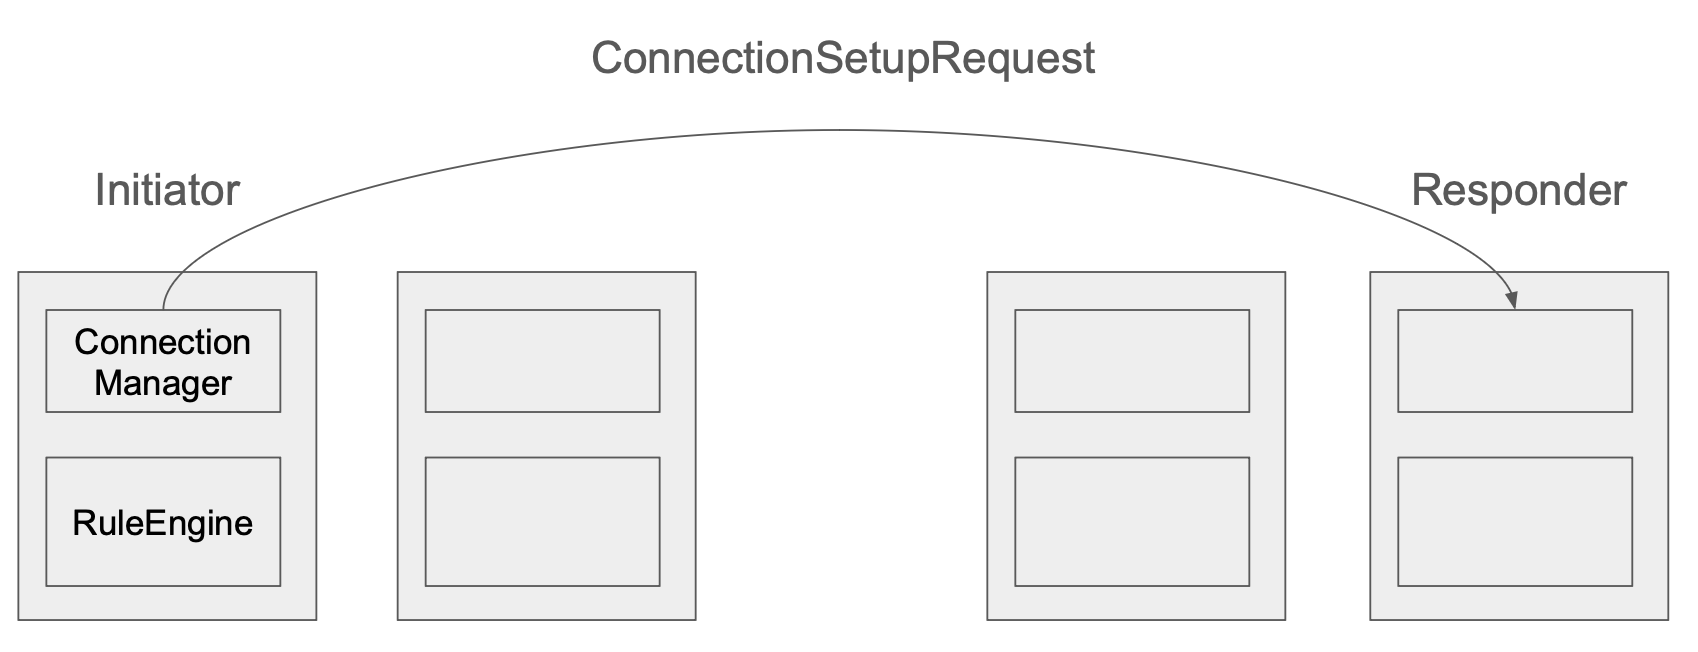
\includegraphics[width=\columnwidth]{images/connection_setup_request.png}}
  \caption{Transmission of a ConnectionSetupRequest}
\end{figure}

After the responder receives ConnectionSetupRequest, it sends Ack and RuleSet to each node along the path of the connection.
\begin{figure}[H]
  \centerline{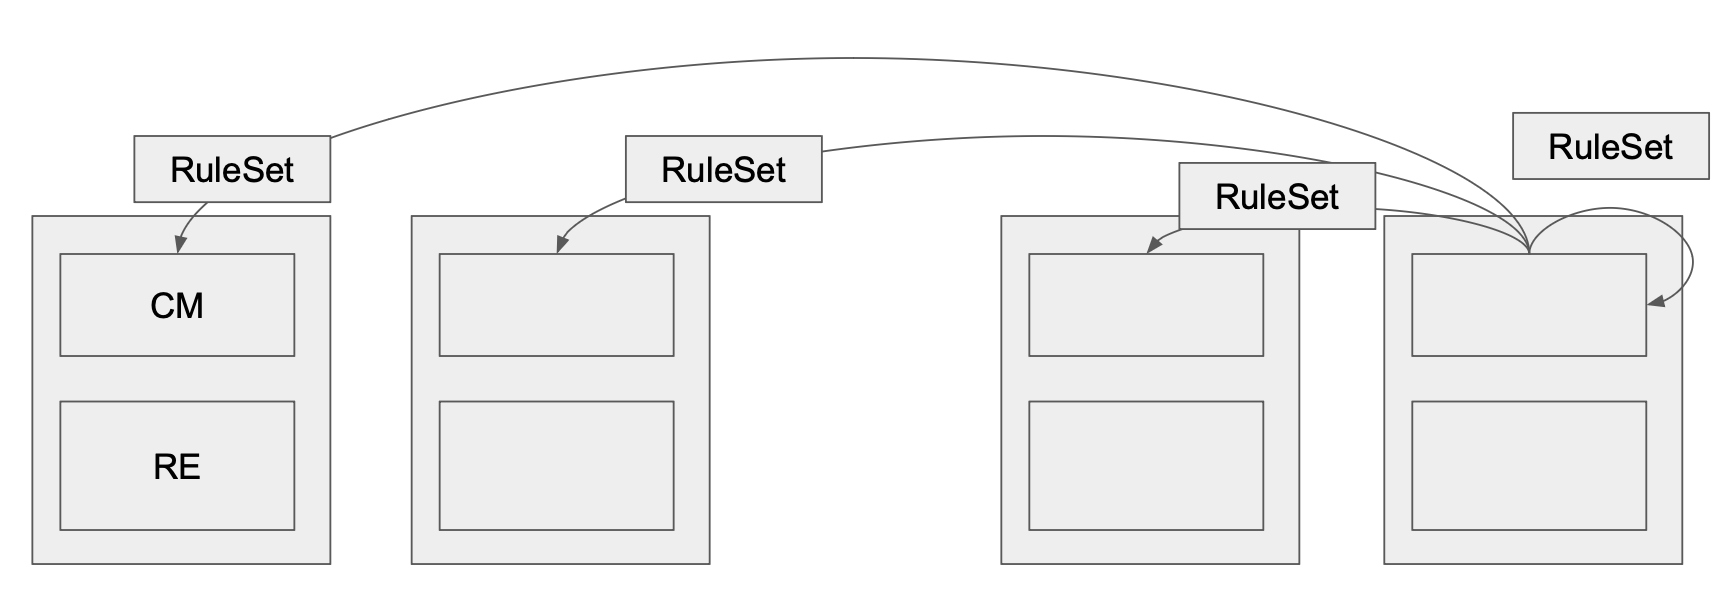
\includegraphics[width=\columnwidth]{images/ack_and_ruleset.png}}
  \caption{Transmission of RuleSets}
\end{figure}

The RuleSet received by the ConnectionManager will be stored in RuleEngine in each node.
\begin{figure}[H]
  \centerline{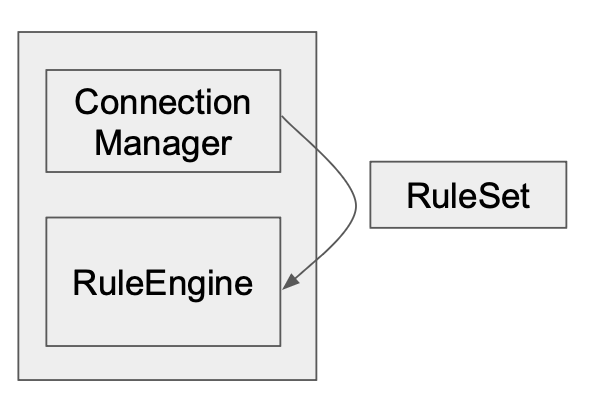
\includegraphics[width=0.7\columnwidth]{images/ruleset_in_rule_engine.png}}
  \caption{Storing RuleSet in the RuleEngine}
\end{figure}

The reception of RuleSet triggers the transmission of LinkAllocationUpdateMessage to each of the neighboring nodes.
After each node both sent and received LinkAllocationUpdateMessages, it determines the next link allocation policy with each of the neighboring nodes.
\begin{figure}[H]
  \centerline{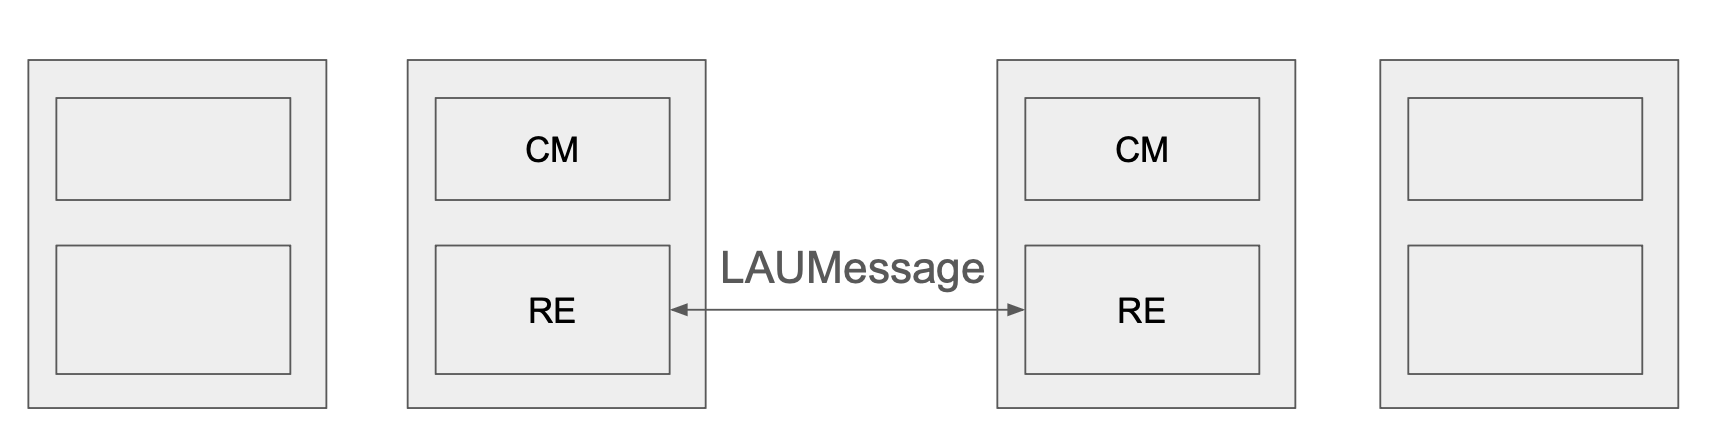
\includegraphics[width=\columnwidth]{images/lau_negotiation.png}}
  \caption{Exchange of LinkAllocationUpdateMessages}
\end{figure}

Generation of link Bell pairs are performed independently from exchange of messages.
\begin{figure}[H]
  \centerline{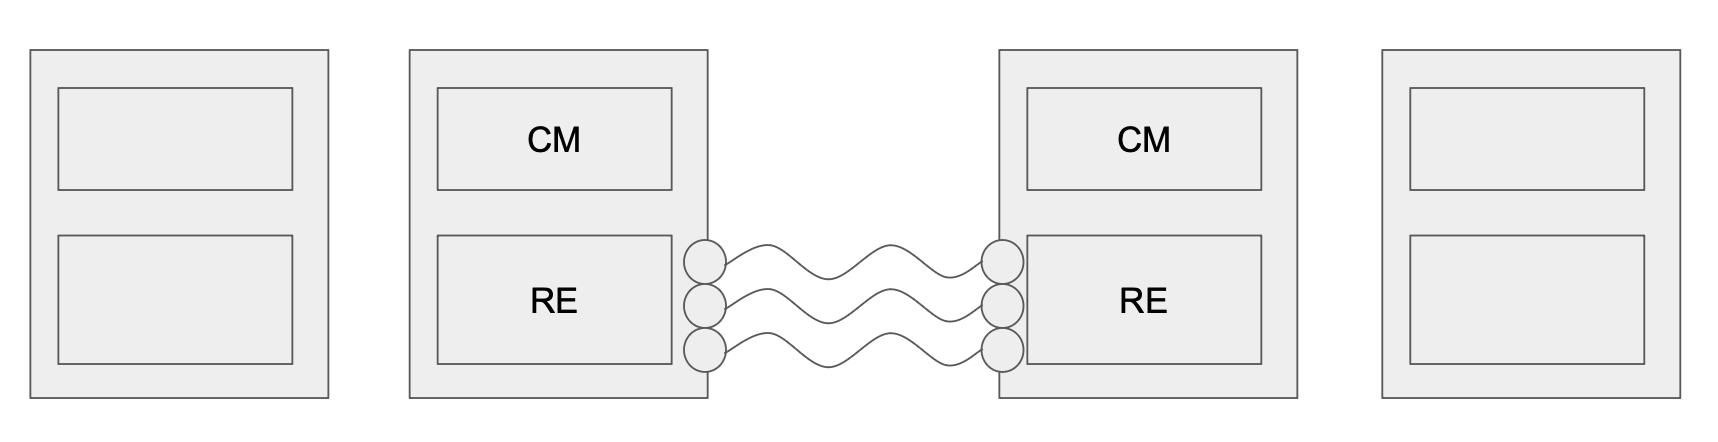
\includegraphics[width=\columnwidth]{images/bell_pair_generation.png}}
  \caption{Generation of Link-level Bell pairs}
\end{figure}

BarrierMessages will be exchanged only if the next link allocation policy is determined and available link Bell pairs exist with each of the neighboring nodes.
After each node sent and receives BarrierMessages, the first sequence number for the next link allocation is determined.
\begin{figure}[H]
  \centerline{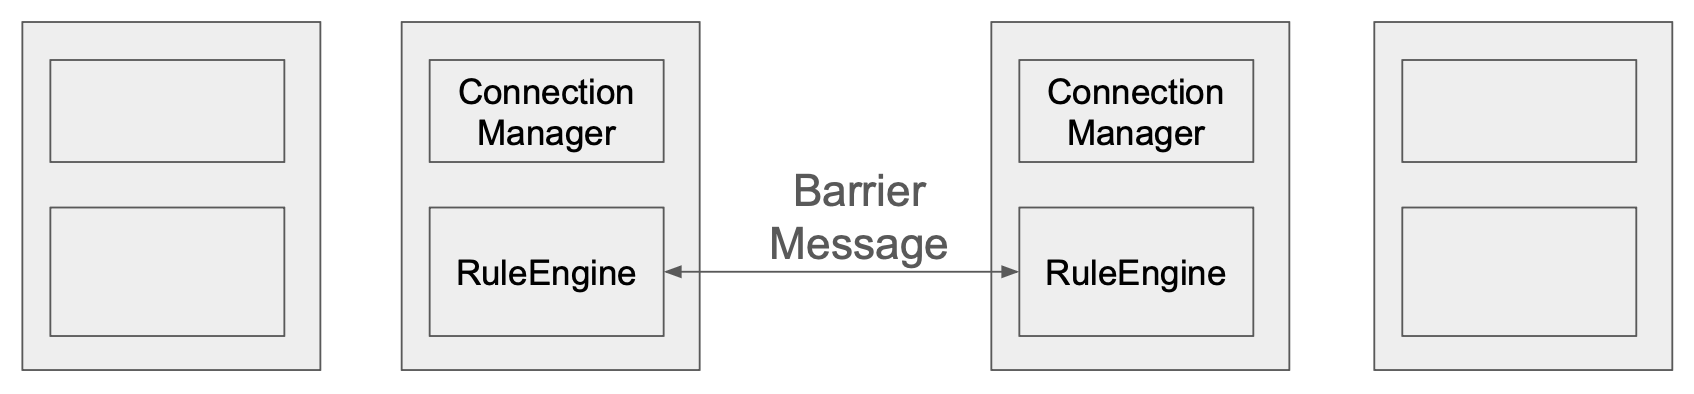
\includegraphics[width=\columnwidth]{images/barrier_negotiation.png}}
  \caption{Exchange of BarrierMessages}
\end{figure}

the first sequence number for the next link allocation is negotiated, each link Bell pairs will be allocated to one of the runtimes for the RuleSets in the next link allocation policy.
\begin{figure}[H]
  \centerline{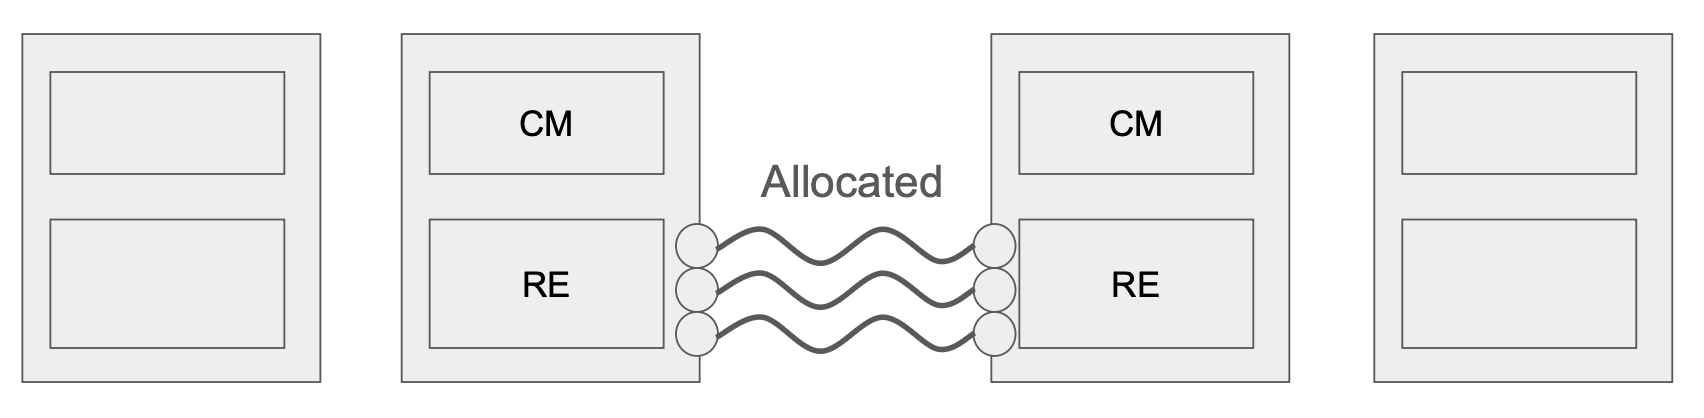
\includegraphics[width=\columnwidth]{images/link_allocation.png}}
  \caption{Allocation of Link Bell pairs}
\end{figure}

\subsubsection{Connection Teardown}

After the RuleEngine detects the termination of execution of the RuleSet, the responder sends a ConnectionTeardownNotifier to its ConnectionManager.
\begin{figure}[H]
  \centerline{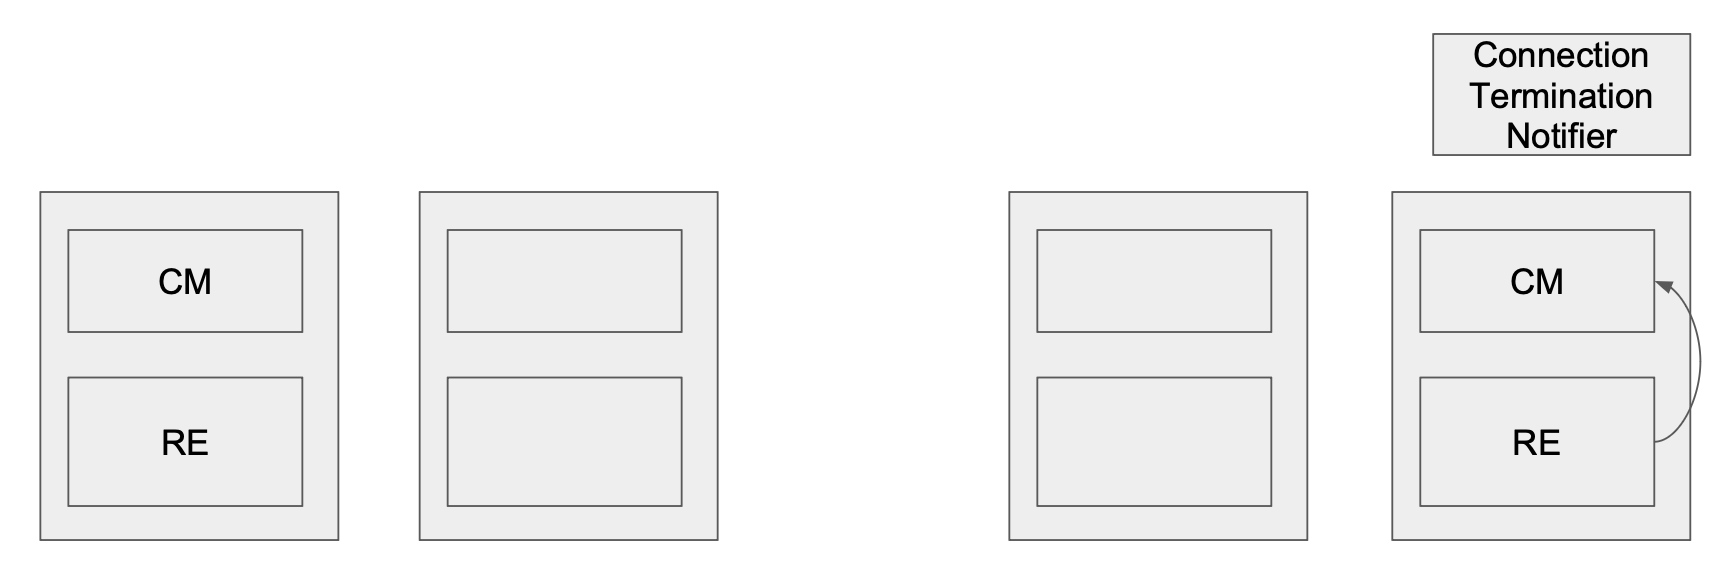
\includegraphics[width=\columnwidth]{images/connection_teardown_notifier.png}}
  \caption{Transmission of ConnectionTeardownNotifier}
\end{figure}

After the ConnectionManager receives a ConnectionTeardownNotifier, it sends a ConnectionTeardownMessage to each node along the path of the connection.

\begin{figure}[H]
  \centerline{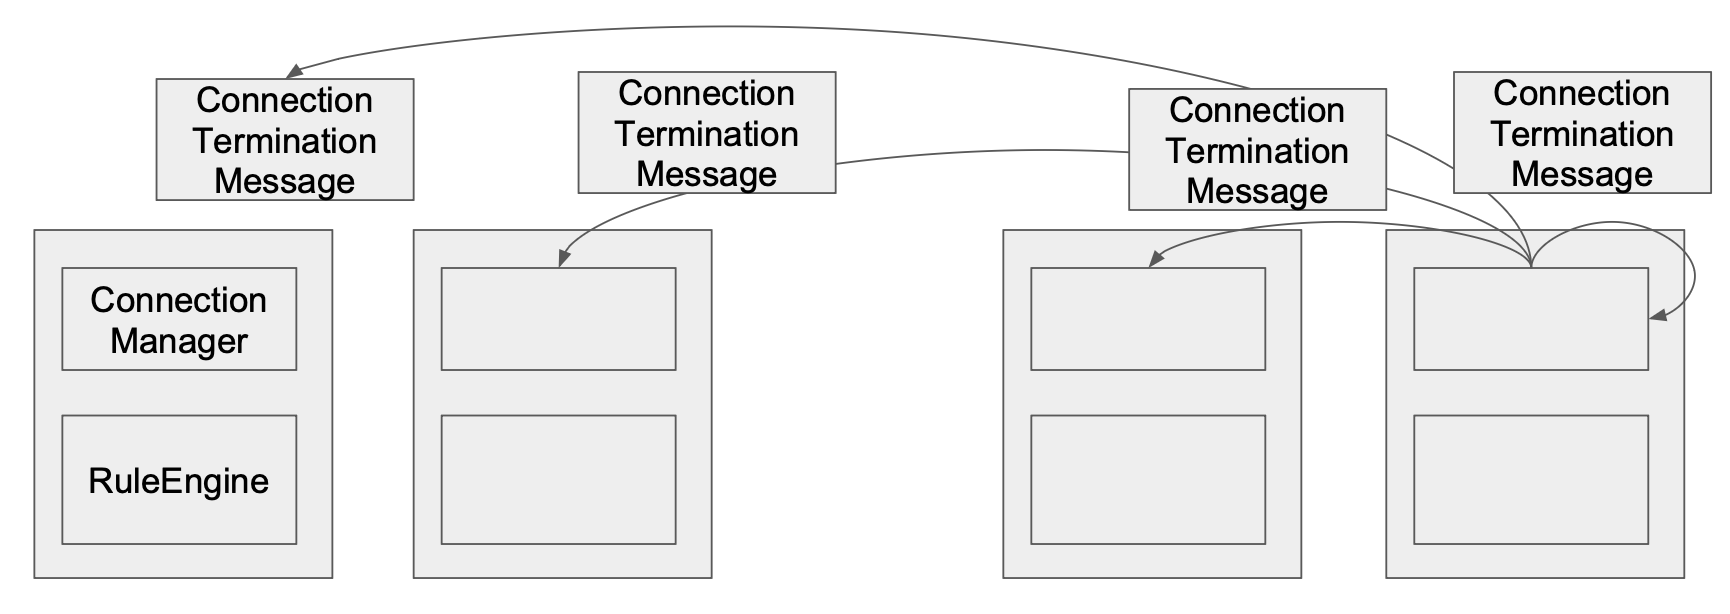
\includegraphics[width=\columnwidth]{images/connection_teardown_message.png}}
  \caption{Transmission of ConnectionTeardownMessages}
\end{figure}

After each node receives a ConnectionTeardownMessage, it stores the message to the RuleEngine in the same node.
The name of the message is changed to an InternalConnectionTeardownMessage for a better readability.

\begin{figure}[H]
  \centerline{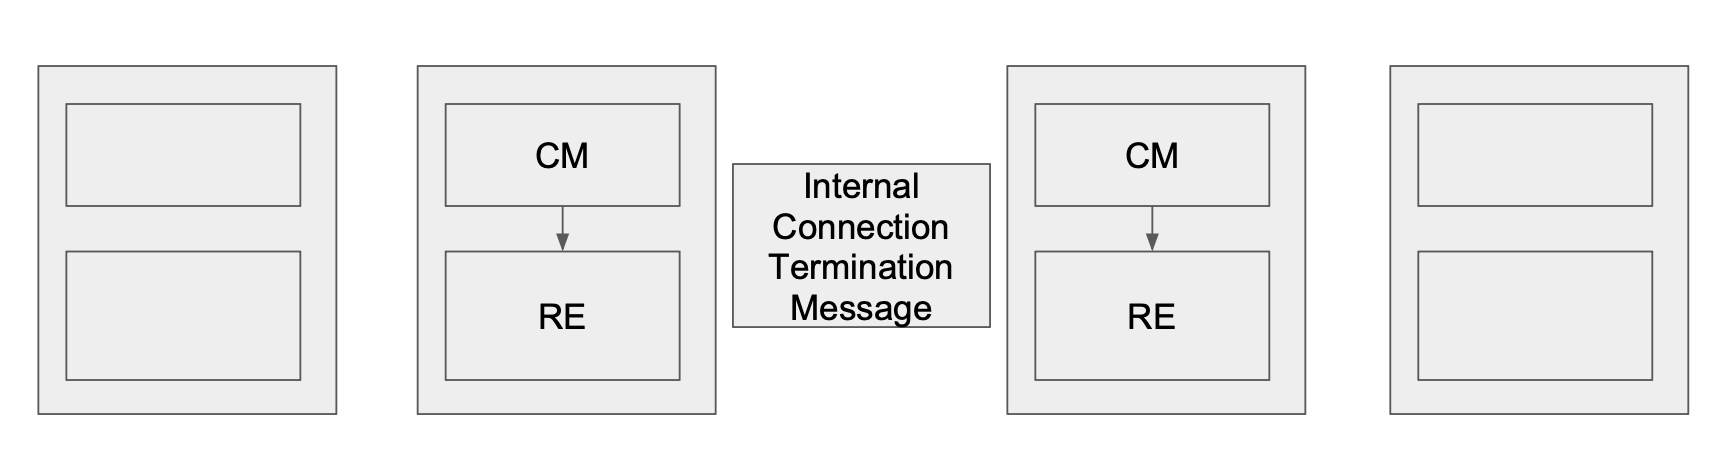
\includegraphics[width=0.7\columnwidth]{images/internal_connection_teardown_message.png}}
  \caption{Storing a ConnectionTeardownMessage}
\end{figure}

After the RuleEngine receives an InternalConnectionTeardownMessage, it terminated the execution of the RuleSet for the connection that was torn down.

\begin{figure}[H]
  \centerline{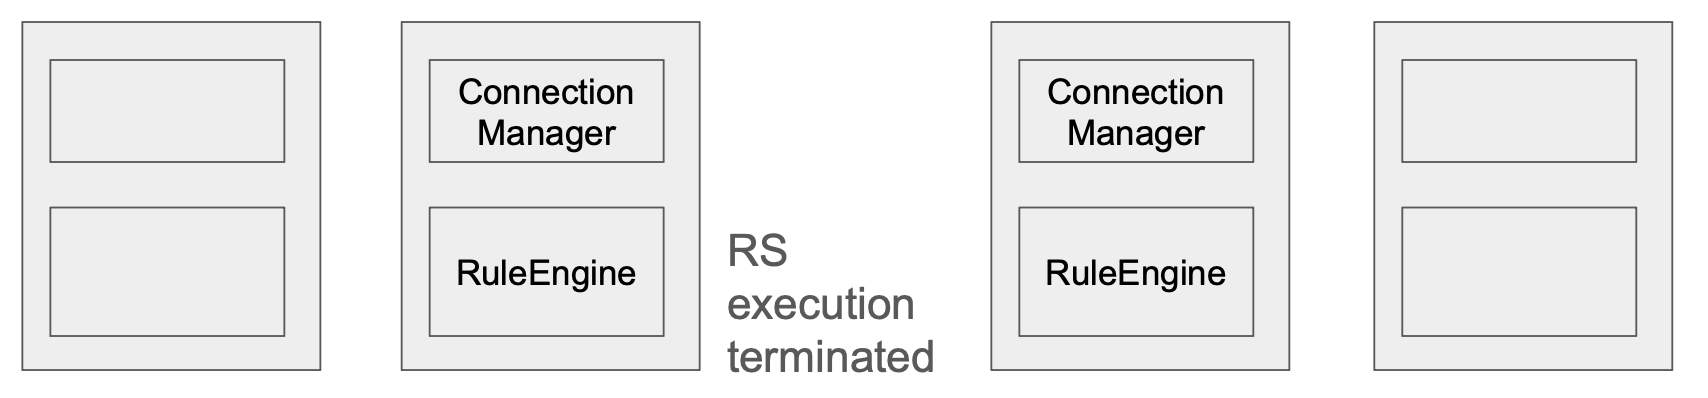
\includegraphics[width=\columnwidth]{images/ruleset_execution_terminated.png}}
  \caption{Termination of the execution of RuleSets}
\end{figure}

Lastly, all the link-level Bell pairs that are allocated but not consumed are released so that they can be reused for new RuleSets.

\begin{figure}[H]
  \centerline{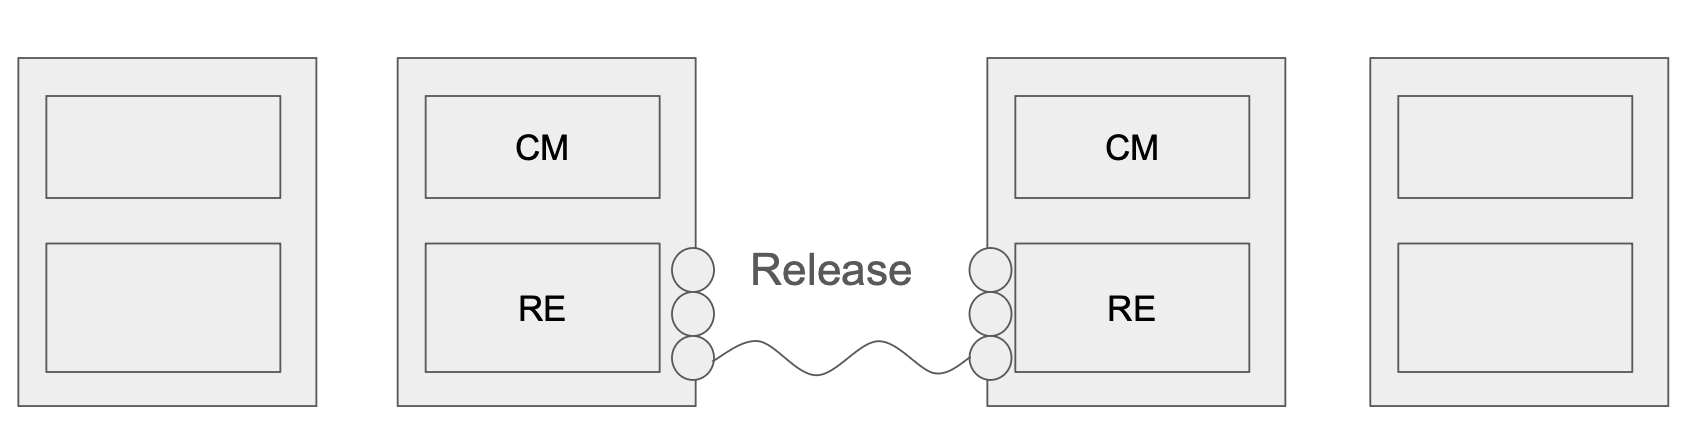
\includegraphics[width=\columnwidth]{images/link_release.png}}
  \caption{Release of allocated Link Bell pairs}
\end{figure}


%%% Local Variables:
%%% mode: japanese-latex
%%% TeX-master: "../bthesis"
%%% End:
